\chapter[Estimating the Effects of Monetary Policy]{Estimating the Effects of Monetary Policy\raisebox{.3\baselineskip}{\normalsize\footnotemark}}
\footnotetext{All equations are important in this chapter, so I did not highlight them one-by-one.}

\fancyhead[L]{ECON0024}
\fancyhead[C]{Ch.8 Estimating the Effects of Monetary Policy}
\fancyhead[R]{Xiaotian Tian}
\fancyfoot[L]{\hyperlink{tableofcontents}{Back to Table of Contents}}
\fancyfoot[R]{Xiaotian Tian}

\section{Introduction}

    We need to evaluate the effectiveness of monetary policies, but face the following difficulties:
    
    \begin{itemize}
        \item We cannot conduct RCTs for monetary policies due to feasibility and morality reasons
        \item We cannot rely on natural experiments because there will be no "control group"
    \end{itemize}

    Therefore, we resort to econometric strategies and assumptions. We cannot simply regress outcomes on changes in interest rates due to endogeneity (simultaneity, feedback, etc.), and this will not inform us about the effectiveness of unconventional policies.

\section{$\star$ Vector Auto-Regression (VAR)}

    \subsection{Vector Auto-Regression (VAR) Models}

        An AR(p) model:
        \begin{equation*}
            y_t = \alpha_y + \beta_1 y_{t-1} + \beta_2 y_{t-2} + \dots + \beta_p y_{t-p} + u_{y,t}
        \end{equation*}

        We can extend this by adding other covariates, and this forms an \emphb{Auto-regressive Distributed Lag} (ADL) Model.

        \begin{equation}
            \begin{split}
                y_t = \alpha_y &+ \underbrace{\beta_{y,1} y_{t-1} + \beta_{y,2} y_{t-2} + \dots + \beta_{y,p} y_{t-p}}_{\text{Lags of } y}\\ &+
                \underbrace{\beta_{x,1} x_{t-1} + \beta_{x,2} x_{t-2} + \dots + \beta_{x,p} x_{t-p}}_{\text{Lags of } x} \\ &+ \underbrace{\beta_{z,1} z_{t-1} + \beta_{z,2} z_{t-2} + \dots + \beta_{z,p} z_{t-p}}_{\text{Lags of } z} + u_{y,t}
            \end{split}
            \label{eqn:ADL}
        \end{equation}
        
        Express this equation (\ref{eqn:ADL}) in its vector form:

        \begin{equation}
            y_t = \alpha_y + \sum_{l=1}^p \begin{pmatrix}
                \beta_{l,y}, & \beta_{l,x}, & \beta_{l,z}
            \end{pmatrix}
            \begin{pmatrix}
                y_{t-l}\\
                x_{t-l}\\
                z_{t-l}
            \end{pmatrix}
            +u_{y,t}
            \label{eqn:ADL vector}
        \end{equation}

        Apply this vector form of ADL model (\ref{eqn:ADL vector}) to inflation $\pi_t$, unemployment rate $U_t$, and interest rate $r_t$:

        \begin{equation}
            \begin{cases}
            
            \pi_t = \alpha_\pi + \sum_{l=1}^p \begin{pmatrix}
                \beta_{l,\pi}, & \beta_{l,U}, & \beta_{l,r}
            \end{pmatrix}&
            \begin{pmatrix}
                \pi_{t-l}\\
                U_{t-l}\\
                r_{t-l}
            \end{pmatrix}
            +u_{\pi,t}\\
            
            U_t = \alpha_U + \sum_{l=1}^p \begin{pmatrix}
                \rho_{l,\pi}, & \rho_{l,U}, & \rho_{l,r}
            \end{pmatrix}&
            \begin{pmatrix}
                \pi_{t-l}\\
                U_{t-l}\\
                r_{t-l}
            \end{pmatrix}
            +u_{U,t}\\
            
            r_t = \alpha_r + \sum_{l=1}^p \begin{pmatrix}
                \gamma_{l,\pi}, & \gamma_{l,U}, & \gamma_{l,r}
            \end{pmatrix}&
            \begin{pmatrix}
                \pi_{t-l}\\
                U_{t-l}\\
                r_{t-l}
            \end{pmatrix}
            +u_{r,t}
            \end{cases}
            \label{eqn:ADL vector system}
        \end{equation}

        Again, stack the three equations in \ref{eqn:ADL vector system} vertically into a \emphb{Vector Auto-Regression} (VAR) model:

        \begin{equation}
            \underbrace{
            \begin{pmatrix}
                \pi_t\\
                U_t\\
                r_t
            \end{pmatrix}}_{Y_{t,3\times 1}}
            =
            \underbrace{
            \begin{pmatrix}
                \alpha_{\pi}\\
                \alpha_{U}\\
                \alpha_{r}
            \end{pmatrix}}_{\alpha_{3\times 1}}
            +
            \sum_{l=1}^p \left\{
            \underbrace{
            \begin{pmatrix}
                \beta_{l,\pi}, & \beta_{l,U}, & \beta_{l,r}\\
                \rho_{l,\pi}, & \rho_{l,U}, & \rho_{l,r}\\
                \gamma_{l,\pi}, & \gamma_{l,U}, & \gamma_{l,r}
            \end{pmatrix}
            }_{B_{l,3\times 3}}
            \underbrace{
            \begin{pmatrix}
                \pi_{t-l}\\
                U_{t-l}\\
                r_{t-l}
            \end{pmatrix}}_{Y_{t-l,3\times 1}}
            \right\}
            +
            \underbrace{
            \begin{pmatrix}
                u_{\pi,t}\\
                u_{U,t}\\
                u_{r,t}
            \end{pmatrix}}_{u_{t,3\times 1}}
            \label{eqn:VAR}
            \tag{VAR}
        \end{equation}
            
        \begin{equation*}
            Y_{t,3\times 1}=\alpha_{t,3\times 1}+\sum_{l=1}^p \Big\{ B_{l,3\times 3} Y_{t-l,3\times 1} \Big\} + u_{t,3\times 1}
        \end{equation*}

        Simple VARs like this are useful for forecasting.

    \subsection{Impulse Response Functions}

        An \emphb{Impulse Response Function} (IRF) is the change in one variable associated with a change in another at some lag, which is the cornerstone of empirical macroeconomics.

        Conceptually, we think of these as a response of $Y_{t+h}$ to a change in $u_{j,t}$, because changing $u_{j,t}$ does affect variables in previous periods.

        \begin{itemize}
            \item A contemporary ($h=0$) IRF of a change in $u_{j,t}$ is:
            \begin{equation*}
                \Phi_j^0 = \frac{\partial Y_t}{\partial u_{j,t}} = \iota_j
            \end{equation*}
            where $\iota_j$ is a vector with 1 in the $j$th entry and 0 otherwise.
            \item IRF ($\Phi$) at horizon $h$ can be computed recursively from knowledge of $B_1,\dots, B_p$:
            \begin{equation*}
            \Phi_j^h = \sum_{k=1}^{min(p,h)} B_k \Phi_j^{h-k} = \sum_{k=1}^{min(p,h)} B_k \frac{\partial Y_t}{\partial u_{j,t-h+k}}
            \end{equation*}
        \end{itemize}

\section{$\star$ Causal Analysis and Structural VAR (SVAR)}

    \subsection{A Conceptual Framework for Causal Analysis}

        We want to study responses to changes in policy that are \emph{unpredictable}.
        
        If it is predictable:
        \begin{itemize}
            \item The estimated effects are caused by whatever predicts the policy
            \item Rational gents have already responded to the anticipated policy change
        \end{itemize}

        Formally, a change is \emphb{endogenous} if it is predicted or caused by another change. A change is \emphb{exogenous} if it is unpredictable and not a causal result of something else. A movement in a macroeconomic time series that is exogenous is a \emphb{structural shock}. We want to study those structural shocks as as-if random variations in policy, or surprises.

    \subsection{Structural VAR (SVAR) Models}

        \subsubsection{Setup}
        
            The vector of VAR residuals $u_i$ is unpredictable but they are \emph{not shocks} because they are cross-correlated, and they are \emph{endogenous}. Exogenous shock should be uncorrelated.
    
            The \emphb{Structural VAR} (SVAR) model assumes the residuals $u_t$ in \ref{eqn:VAR} as linear combinations of $n$ unobserved uncorrelated shocks $\epsilon_t$ (\emphb{SVAR assumption 1}). With this, we rewrite the \ref{eqn:VAR} equation:
    
            \begin{equation}
                \underbrace{
                \begin{pmatrix}
                    \pi_t\\
                    U_t\\
                    r_t
                \end{pmatrix}}_{Y_{t,3\times 1}}
                =
                \underbrace{
                \begin{pmatrix}
                    \alpha_{\pi}\\
                    \alpha_{U}\\
                    \alpha_{r}
                \end{pmatrix}}_{\alpha_{3\times 1}}
                +
                \sum_{l=1}^p \left\{
                \underbrace{
                \begin{pmatrix}
                    \beta_{l,\pi}, & \beta_{l,U}, & \beta_{l,r}\\
                    \rho_{l,\pi}, & \rho_{l,U}, & \rho_{l,r}\\
                    \gamma_{l,\pi}, & \gamma_{l,U}, & \gamma_{l,r}
                \end{pmatrix}
                }_{B_{l,3\times 3}}
                \underbrace{
                \begin{pmatrix}
                    \pi_{t-l}\\
                    U_{t-l}\\
                    r_{t-l}
                \end{pmatrix}}_{Y_{t-l,3\times 1}}
                \right\}
                +
                \underbrace{
                \begin{pmatrix}
                    A_{11}, & A_{12}, & A_{13}\\
                    A_{21}, & A_{22}, & A_{23}\\
                    A_{31}, & A_{32}, & A_{33}
                \end{pmatrix}
                }_{A_{3\times 3}}
                \underbrace{
                \begin{pmatrix}
                    \epsilon_1\\
                    \epsilon_2\\
                    \epsilon_3
                \end{pmatrix}}_{\epsilon_{t,3\times 1}}
                \label{eqn:SVAR}
                \tag{SVAR}
            \end{equation}
            
            \begin{equation*}
                Y_t = \alpha + \sum_{l=1}^p B_l Y_{t-l} + \underbrace{A\epsilon_t}_{u_t}
            \end{equation*}
            
            and the shocks are:
            
            \begin{itemize}
                \item $E[\epsilon_t]=0$ (has zero mean)
                \item $E[\epsilon_t \epsilon_t']=I_n$ (has unit variance and zero covariance)
                \item $E[\epsilon_t \epsilon_s]=0$ (no serially correlated)
            \end{itemize}
    
            The full-rank matrix $A$ is the \emphb{Contemporaneous Response Matrix}. $A_{ij}$ us the effect of a unit shock $j$ on variable $i$ instantly, which is interpreted causally.

        \subsubsection{Estimate the Effects of Shocks with Assumptions}

            $E[u_t]=AE[\epsilon_t]=A\times 0=0$ informs us nothing.\\
            $Cov(u_t)=E[u_tu_t']=AE[\epsilon_t\epsilon_t']A'=AA'$ There are $n(n+1)/2$ equations with $n^2$ unknowns, so we need additional $n(n-1)/2$ restrictions to find a unique solution.

            The further assumptions restraining the unknowns (\emphb{SVAR assumption 2}) take the simplest form of recursive/timing restrictions: we restrict which variables can respond to which shocks contemporaneously. Technically, we impose that:
            \begin{equation}
                A=\begin{pmatrix}
                A_{11} & 0 & 0\\
                A_{21} & A_{22} & 0\\
                A_{31} & A_{32} & A_{33}
            \end{pmatrix}
            \label{eqn:SVAR_assumption_2}
            \tag{SVAR Assumption 2}
            \end{equation}
            
            With ordering $Y_t=\begin{pmatrix}
                \pi_t\\
                U_t\\
                r_t
            \end{pmatrix}$, these restrictions means:
            \begin{itemize}
                \item Inflation only responds to price shocks contemporaneously
                \item Unemployment responds to both price and labour market (unemployment) shocks contemporaneously
                \item Interest rate responds to all price, labour market (unemployment), and monetary policy (interest rate) shocks contemporaneously
            \end{itemize}
            
            Under these restrictions , $A$ is the unique lower triangular \emphb{Cholesky factor} of $Cov(u_t)=E[u_tu_t']=AA'$, and all its entries can be estimated.

        \subsubsection{Structural Impulse Responses}

            After estimated the corresponding coefficients in SVAR, we can cumpute the \emphb{structural impulse responses} -- the \emph{dynamic causal effects} of monetary policy.

            The structural impulse response of a structural shock $\epsilon_j$ as time $t$ on variable $Y$ at time $t+h$ is:
            \begin{align*}
                \Theta_j^h &= \frac{\partial Y_{t+h}}{\partial \epsilon_{j,t}}\\
                &= \frac{\partial Y_{t+h}}{\partial u_t'}\frac{\partial u_t}{\partial \epsilon_{j,t}} \tag{Product Rule}\\
                &=\Phi^h A_{.j}
            \end{align*}
            where $\Phi^h$ is the $h$ period IRF, and $A_{.j}$ is the $j$th row of $A$.
            
    \section{$\star$ Alternatives to SVAR}
    
        \subsection{Alternative Restrictions}

            The timing assumptions we used (\ref{eqn:SVAR_assumption_2}) are very strong, so we may want to use others:
            \begin{itemize}
                \item \emphb{Long-run Restrictions}: assume effects of some shocks die out at long horizons
                \item \emphb{Sign Restrictions}: assume some elements in $A$ have certain signs (e.g. interest hike lowers inflation). This rules out some solutions for $A$ and gives us \emph{a range of possible values}, but not unique point estimates.
            \end{itemize}
            
        \subsection{Alternative Method: Instrumental Variables}

            Still using the structure of \ref{eqn:SVAR}, we can use \emphb{instrumental variables} (e.g. an instrument that is correlated with monetary policy shock but not price or labour market shocks) to estimate the corresponding column of $A$.

            To implement this, we regress each series in $u_t$ on instrument $z_t$ by OLS, then normalise the vector of coefficients by the coefficient of $u_{r,t}$ to get $A_{mp}$.

        \subsection{Alternative Method: Local Projections (LP)}

            \subsubsection{Local Projections}
            
                \emphb{Local Projection (LP)} is an alternative method to estimate the effects of monetary policy (or other macro policies). Generally, this is more flexible than VARs. LPs are direct OLS regressions to forecast some outcome:
                \begin{equation}
                    y_{t+h}-y_{t-1}=a+\lambda_hr_t+\sum_{l=1}^p \kappa_l X_{t-l} +v_t
                    \tag{Local Projections}
                \end{equation}
                where $X_{t-l}$ is a set of controls (inflation, unemployment, etc.)
                
                The IRF at horizon $h$ is simply $\lambda_h$. However, note that, because $r_t$ is likely to be endogenous, $\lambda_h$ does not have a causal interpretation yet. It is just the response to the part of $r_t$ that is unpredictable by $X_{t-1}, \dots, X_{t-p}$.

            \subsubsection{Local Projections with Instrumental Variables}
            
                To deal with endogeneity and obtain causal responses, LPs are always implemented with \emphb{instrumental variables}.

                The implementation is just like 2SLS:
                \begin{itemize}
                    \item First stage: regress $r_t$ on IV $z_t$ and controls (lags of $X$); predict $\hat{r}_t$
                    \item Second stage: regress $(y_{t+h}-t_{t-1})$ on $\hat{r}_t$ and controls (lags of $X$)
                \end{itemize}
                $\lambda_h$ estimated in the second stage is the dynamic causal effect at horizon $h$.

                When choosing instruments, as usual, we need to ensure exogeneity and relevance. Adding controls can help with their validity. Some examples of IV: high frequency financial data and "narrative" rate changes regressed on internal CB forecasts.

                In general, we should not use measured shocks directly as independent variables (regressors), because there are measurement errors and scaling issues.

    \section{Empirical Findings}

        \subsection{Literatures}

            \begin{figure}[H]
                \centering
                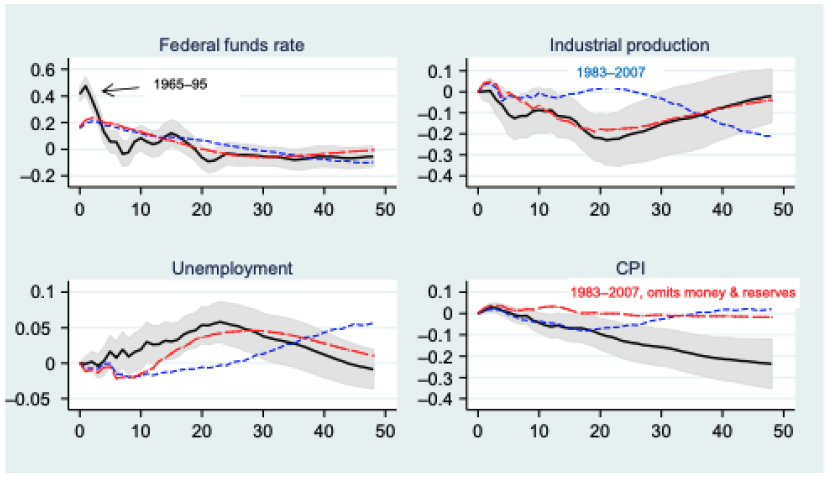
\includegraphics[width=4in]{images/ch8/mp_christiano.png}
                \caption{Christiano, Eichenbaum, \& Evans (1999): Recursive SVAR (Lower Triangle)}
            \end{figure}
            \begin{figure}[H]
                \centering
                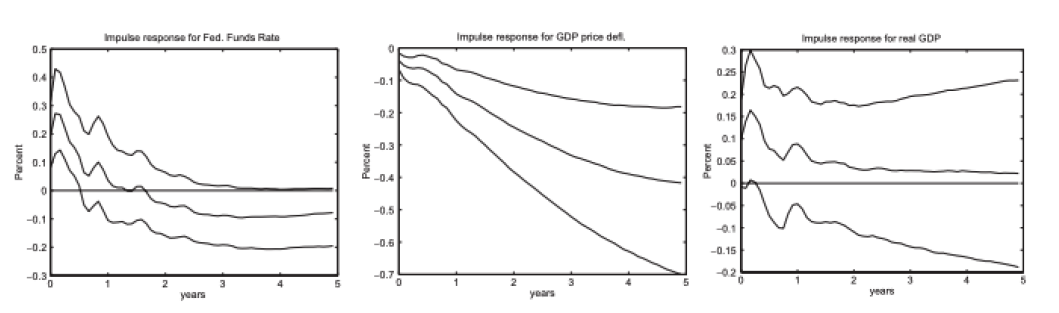
\includegraphics[width=5in]{images/ch8/mp_Uhlig.png}
                \caption{Uhlig (2005): SVAR with Sign Restrictions}
            \end{figure}
            \begin{figure}[H]
                \centering
                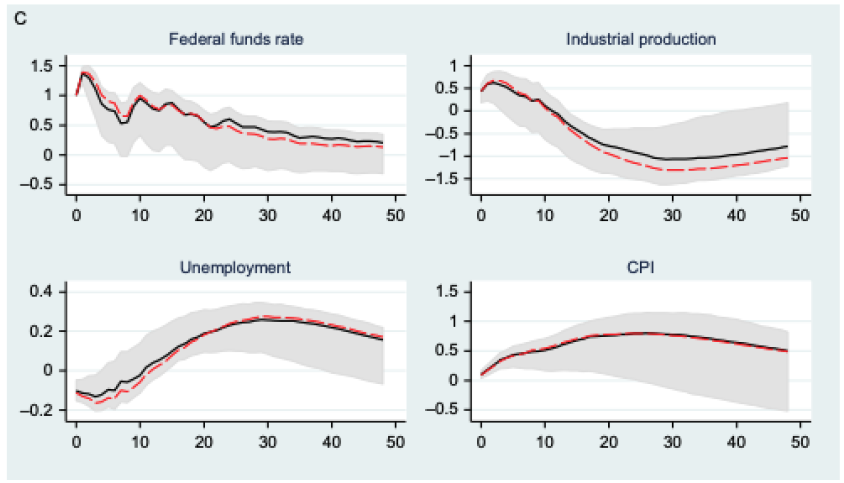
\includegraphics[width=4in]{images/ch8/mp_Romer.png}
                \caption{Romer \& Romer (2004): SVAR with Instrumental Variables}
            \end{figure}
            \begin{figure}[H]
                \centering
                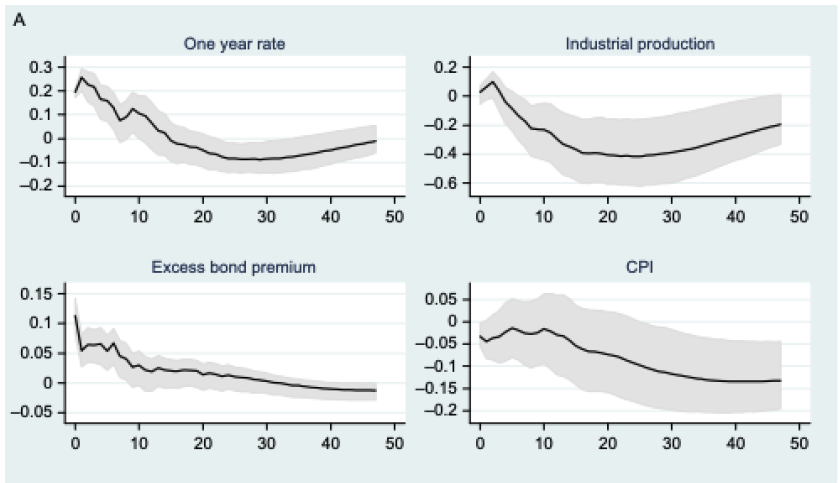
\includegraphics[width=4in]{images/ch8/mp_Gertler.png}
                \caption{Gertler \& Karadi (2015): SVAR with Instrumental Variables}
            \end{figure}
            \begin{figure}[H]
                \centering
                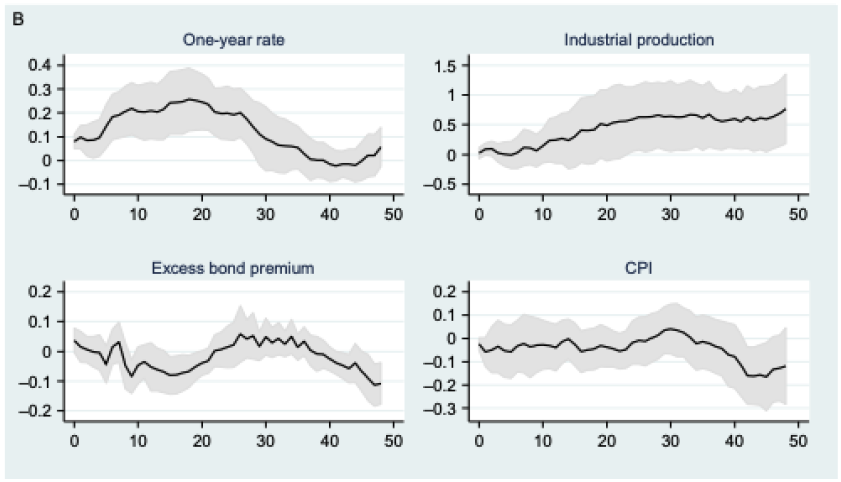
\includegraphics[width=4in]{images/ch8/mp_Gertler_LP.png}
                \caption{Gertler \& Karadi (2015): Local Projections (LP) with Instrumental Variables}
            \end{figure}
            
        \subsection{Evaluating Macroeconometric Models}
            When estimating causal effects in macroeconomic settings, there is no "truth":
            \begin{itemize}
                \item There is no single way to estimate effects even given the same dataset
                \item Results are sensitive to restrictions/assumptions imposed
                \item Also, typically, assumptions cannot be tested, because we cannot estimate the model at all without assumptions
            \end{itemize}
            Therefore, it is important to think about \emphb{robustness}: are there findings that are relatively insensitive to alternative assumptions? (i.e. looking for common findings)

        \subsection{Effectiveness of Monetary Policy}

            \subsubsection{Conventional Monetary Policy}

                \begin{figure}[H]
                    \centering
                    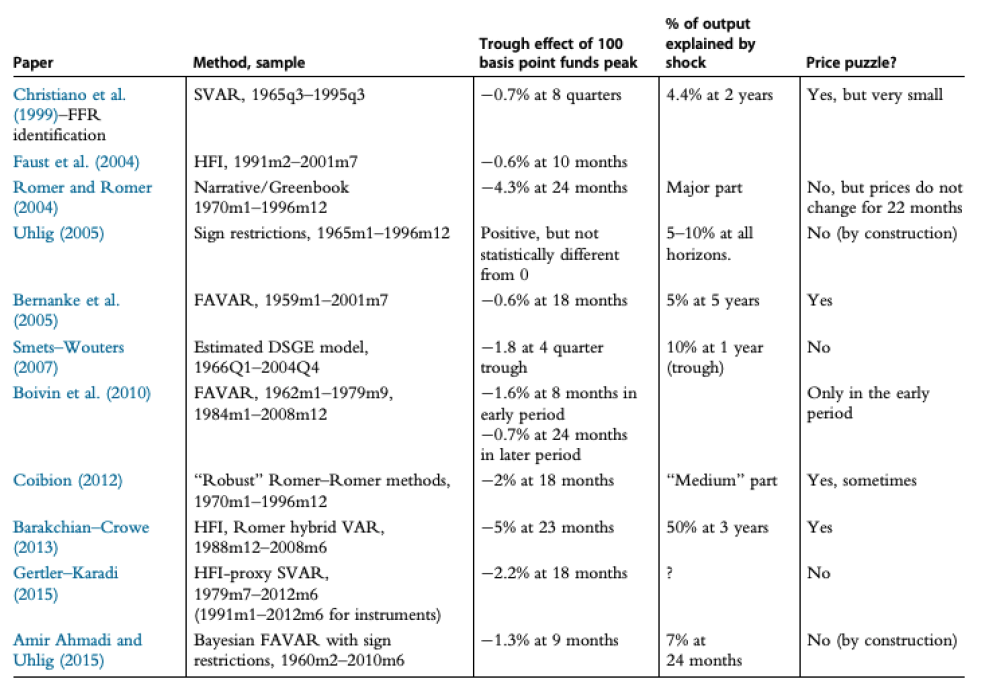
\includegraphics[width=5in]{images/ch8/mp_conclusion.png}
                    \caption{Summary of Leading Results (Ramey (2016))}
                \end{figure}
                The answers are surprisingly tentative. In many empirical macroeconomics literatures (half of the examples shown above), we saw the \emphb{price puzzle}: positive interest rate shocks induce higher inflation. Also, response of real activity remains ambiguous with sign restrictions.
            
            \subsubsection{Unconventional Monetary Policy}

                The literature on unconventional policy is still very limited because:
                \begin{itemize}
                    \item For the most part, unconventional policies began in 2008
                    \item Most unconventional policies are short-lived and time-varying, so the sample size is very small
                    \item Sampling period contains a massive recession period, which might not be representative
                \end{itemize}
                Early evidence shows strong effects of some form of forward guidance and asset purchases \emph{on financial markets}. On the other hand, there is less evidence on their effects on most important \emph{macroeconomic variables}: existing evidence suggests that quantitative easing was effective, but forward guidance is less so.

                "QE works in practice, but not in theory."
                
            \subsubsection{Interpretability of Estimates}

                We made some conceptual leaps to recover causal estimates:
                \begin{itemize}
                    \item Structural Shocks: central banks don't set interest rates at random and most of their policies are anticipated by the market. Does central banks have to do something surprising to have an effect, or anticipated changes can also be effective?
                    \item Unrealistic assumptions made
                \end{itemize}
            
        
    